\documentclass[fleqn, 10pt]{article}

% Paquetes necesarios
\usepackage[utf8]{inputenc}
\usepackage{amsthm, amsmath}
\usepackage{nccmath} %Para centrar ecuaciones
\usepackage{graphicx}
\usepackage{amssymb}
\usepackage{enumitem}
\usepackage{ragged2e}

% Personalizo mi alfabeto
\DeclareMathAlphabet{\pazocal}{OMS}{zplm}{m}{n}
\newcommand{\Lb}{\pazocal{L}}

% Definimos los entornos para definiciones, teoremas, etc...
\theoremstyle{plain}
\newtheorem{proposicion}{Proposición}

\theoremstyle{definition}
\newtheorem{definition}{Definición}[section]
\newtheorem{example}{Ejemplo}[section]

%Definimos el título
\title{Teoría de Autómatas y Lenguajes Formales\\[.4\baselineskip]Práctica 4: Numeración de Programas y EXWHILE\\}
\author{Rocío Guzmán Arroyo}
\date{\today}

%Comienzo del documento
\begin{document}

%Generamos el título
\maketitle

\section{Explicación de la Práctica}
Para realizar la practica se nos pide resolver los siguientes ejercicios:

\subsection{Ejercicio 1}

Se nos piede el desarrollo del cálculo de la menor codificación del programa WHILE "diverger".
En otras palabras,lo que se nos pide es la codificación de un codigo WHILE el cuál nunca finaliza.Tiene iteraciones infinitas

\begin{verbatim}

Q : (1, 2, s)
s: 	
X1 := X1 + 1;
while X1 != 0 do
X1 := X1 + 1	
od

\end{verbatim}

Asociamos una condición que nunca se cumple por lo tanto el bucle continua ejecutandose invinitas veces.En tiempos de ejecución una función infinito.

\begin{figure}[h]
\begin{center}
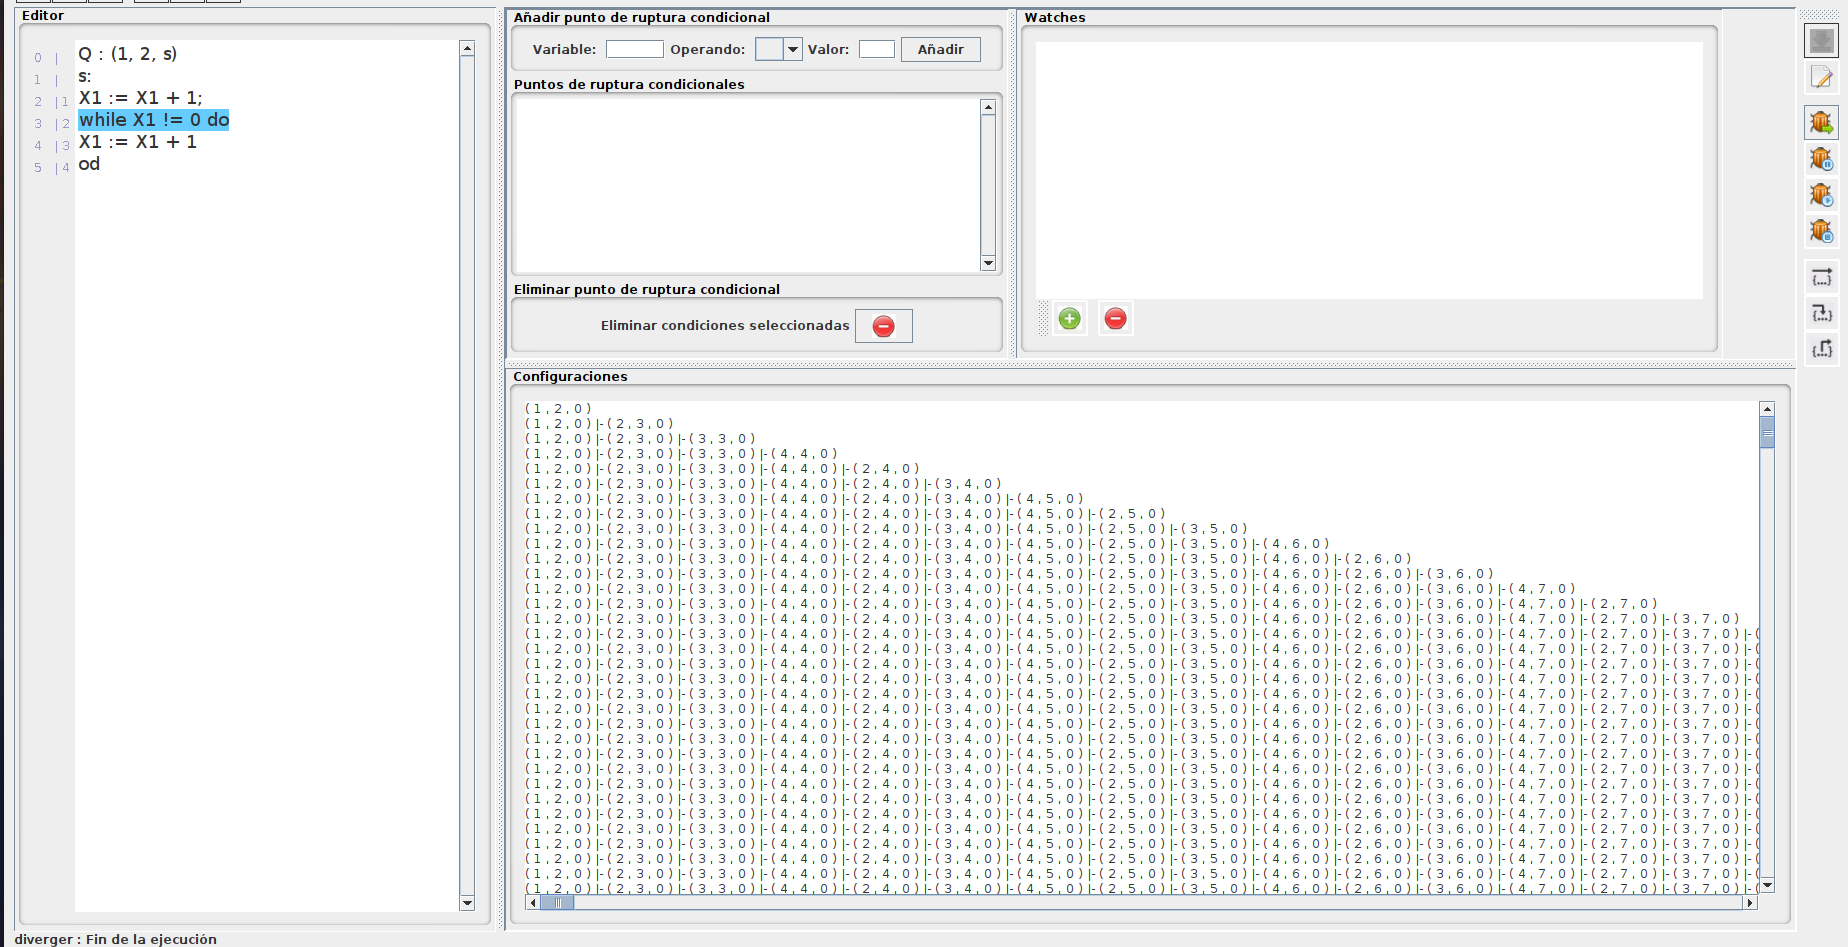
\includegraphics[width=16cm]{Diverger}
\end{center}
\end{figure}

\newpage

\subsection{Ejercicio 2}

Se nos pide un programa en la aplicación 'Octave' que devuelve un número n de vectores que decodifica todos los posibles vectores hasta n.Para esto utilizamos el programa godeldecoding que devuelve la tupla codificada por n.

\begin{figure}[h]

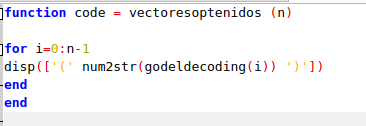
\includegraphics[width=7cm]{Codigo}

\end{figure}

\qquad

En este código simplemente se iterá n veces ya que va de 0 a n-1 vez y aplica el programa godeldecoding.m, es un programa que anteriormente ha sido implementado por el profesor.


\begin{figure}[h]

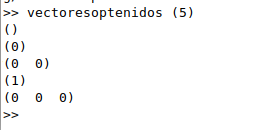
\includegraphics[width=7cm]{Salida}

\end{figure}

\newpage

\subsection{Ejercicio 3}

Debemos implementar un codigo en Octave y adjuntas la salida que proporciona de la misma forma que el código anterior simplemente en este caso lo que devolvemos son los codigos WHILES.


\begin{figure}[h]

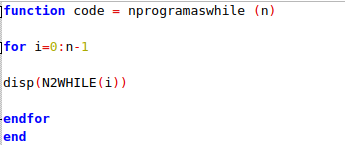
\includegraphics[width=7cm]{Codigo1}

\end{figure}



\begin{figure}[h]

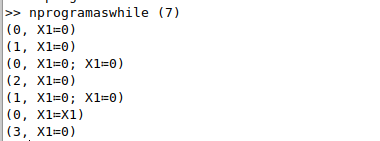
\includegraphics[width=7cm]{Salida1}

\end{figure}

\end{document}